\chapter{Novel \mgii\ Line Profile Comparisons from 1D NLTE Modelling}\label{Chap:prom}


Simulation and modelling are some of the most powerful tools that we have when facing solar atmospheric problems. We cannot directly deduce the conditions of the solar atmosphere with only observations: we need to do some degree of forward modelling. In this chapter we will explore the use of a novel method to find the internal properties of solar prominences. We match line profiles from 1D radiative transfer modelling with that of observed line profiles and use a measure of root mean squared difference (RMS) to evaluate the goodness of fit. From this, we are able to say how confident we are with our matched line profiles and produce maps of the properties of the considered prominence. In this chapter, we will use the 1D non-local thermodynamic equilibrium (NLTE) radiative transfer (RT) code PROM (see \sect{promintro}) to generate models which we wish to match with observation.

\section{Rolling Root Mean Squared (rRMS)}
\textit{The content of this section is based on work presented in section 4 of \cite{peat_solar_2021}.}
\label{rrms}

With these models, we can attempt to invert the solar atmosphere with a grid search. In a grid search, a large group of models of differing parameters is run and then the outputs from the models are subject to some statistical test to determine the model which most closely resembles the observation. In past studies using \ion{Mg}{ii}~h\&k, such as \cite{ruan_diagnostics_2019} and \cite{zhang_launch_2019}, the statistical test employed only concerned the integrated intensities of the lines. In \cite{ruan_diagnostics_2019}, the models and the data were only qualitatively compared by plotting the observed and modelled integrated intensities of \mgii~k against \ha, and  \mgii~h against \ha. It was concluded that these relationships behaved in a consistently similar manner. In \cite{zhang_launch_2019}, the statistical test used was a root mean squared difference (RMS) minimisation between the integrated intensities of the modelled and observed \mgii~h\&k line profiles.

However, these methods discard the most important result of the simulation: the line profiles themselves. It is easy to envision a scenario in which a double peaked profile has the same integrated intensity as a single peaked profile, or vice versa. Directly comparing the modelled line profiles to the observed line profiles allows us to gain a more quantitative result; moreover, we can set a limit on our statistical measure to say whether the fit is acceptable or otherwise. \cite{heinzel_understanding_2015} fitted a computed \mgii\ line profile to the mean of six observed line profiles, but did not extend this idea to every line profile in the observation. Work to fit computed line profiles to every pixel of an observation (on the order of hundreds of thousands of line profiles) by the line shapes seems to have not been undertaken. One of the reasons for this could be that the problem is quite computationally taxing. 

For this problem I developed Rolling RMS (rRMS), which later became Cross RMS (xRMS) where the roll was replaced with a cross-correlation. Currently this works with IRIS data, but could be generalised to work with any spectrograph. Before modelled line profiles can be matched, they first had to be interpolated down to the spectral resolution of the IRIS spectrograph. The spectral pixel resolution of the NUV observations used here is 51~m\AA, while our models have a resolution of 3~m\AA. Initially, this was done through the use of fourth-order weighted essentially non-oscillatory interpolation \citep[WENO4; ][]{janett_novel_2019}\footnote{The Python implementation used can be found at \href{https://github.com/Goobley/Weno4Interpolation}{https://github.com/Goobley/Weno4Interpolation} or installed via pip}, however, it was later found that linear interpolation offered similar results at a greater computational speed. The interpolation was performed such that the models remained symmetrical about their line core. After the models were interpolated down to 51~m\AA, both the models and the data were interpolated up to a resolution of 25.5~m\AA. This was done such that if the line core lay between two spectral pixels in the data, the model profile could be better centred on the data. Tests where the models and data were interpolated up to resolutions of 17~m\AA\ and 12.75~m\AA\ showed that these offered little to no increase in number of matches, whereas the run time increased. The data was trimmed to two separate 3~\AA\ windows centred on the rest wavelengths of \mgii~h\&k, respectively. This spectral window is considerably larger than the wavelength range of the models, and so they are padded with zeros to match the wavelength range of the data. Then, to account for the background level in the observations, the mean of the intensity between 2797.85~\AA{} and 2802.03~\AA{} of the observation is added to the model before matching. These two values are at the edges of the aforementioned 3\AA{} windows. The model line profiles were then rolled through these 3\AA{} wavelength windows measuring the RMS at every position (defined by \eq{rmseq}). See Fig. \ref{fig:rrms} for a visual representation of the algorithm.
\begin{equation}
    \text{RMS}(\Delta\lambda)=\sqrt{\frac{1}{n}\sum_n\left(\text{data}-\text{model}\right)^2},
    \label{rmseq}
\end{equation}
\begin{figure}
    \centering
    \includegraphics*[width=.7956\linewidth]{./02Modelling1D/figs/20180419/rrms1.png}\\
    \includegraphics*[width=.7956\linewidth]{./02Modelling1D/figs/20180419/rrms2.png}
    \caption[Example of rRMS working.]{Example of rRMS working. These panels are in sets of two; with the upper of each set (orange) rolling over the data (blue) and the bottom of each set the current RMS at that position (dotted orange), the future RMS measurements (transparent blue), and the RMS measured up to that point (solid orange). This demonstrates the method employed by the algorithm to find the best fitting location of the currently considered model profile. The model profile is rolled one spectral pixel at a time across the entire wavelength window measuring the RMS at each pixel location.}
    \label{fig:rrms}
\end{figure}

where $n$ is the number of data points in wavelength space. The pixel shift required to produce the lowest RMS is assumed to be the best matching position for that model. The RMS and its associated pixel shift are saved, then the next model is compared. This is done independently for both \mgii~h\&k, then their RMS values are added together and the model that produces the lowest total RMS for that pixel is selected as the model most indicative of the plasma parameters in that pixel. This is done in vectorised fashion through the use of the Numpy Python library \citep{harris_array_2020}, greatly increasing the speed of the computation. Additionally, this was run in parallel over the 18 rasters of the observation on a machine with a dual socket motherboard with two Intel Xeon E5-2697 v4s giving a wall time\footnote{The time taken for the program to execute in real time (i.e., measured by a clock on a wall).} of approximately 1 hour and 30 minutes, and a CPU time\footnote{The sum of the run time on every CPU core/thread.} of 27 hours.

\subsection{Prominence of 2018 04 19}
\label{20180419}
As discussed in section \ref{20180419main}, a prominence appeared off of the south-western solar limb on the 19 April 2018. The observations carried out by IRIS allowed us to develop the aforementioned tool, rRMS. Using the iteration of PROM presented in \cite{levens_modelling_2019}, we generated 1007 model prominences; 252 isothermal and isobaric models, and 755 models with a PCTR. The parameters of these can be seen in table \ref{modeltable}. The parameters here have 1008 unique combinations, however, one of the models did not converge, leaving us with 1007. Here we have one value for both the microturbulent velocity and height parameters. The value used for the microturbulent velocity is the generally accepted value expected to be found in the main bulk of a prominence \citep{labrosse_physics_2010}, however, the latter has a more nuanced argument. Since height is something that can be measured directly from observation, it appears to be something that we can simply feed into our calculations, where every pixel has a height associated with it. In theory, this is  a good idea, but in practice, every new value added to for $H$ will increase the size of the grid by a further 1007 (or 1008 if that one model now converges with a different height). If we assume every pixel in a raster is of the same altitude, we would have to create 32~224 models in total. This is even greater than the extended grid of 23~940 discussed in \sect{xrms}. This may have an effect on the solutions recovered as all of the pixels are not at a height of 10~000~km. At different altitudes, models of similar parameters exhibit lower intensities at higher altitudes. This may mean that higher features may be hotter and/or more dense, and lower features may be cooler and/or less dense. Slab width may also be affected in similar ways.


\begin{table}
    \centering
    \begin{tabular}{ccc}
    \hline \hline
    Parameter & Unit  & Value                                                                \\ \hline\hline
    $T_{\text{cen}}$   & K              & \begin{tabular}[c]{@{}c@{}}6000, 8000, 10~000, 15~000, \\ 20~000, 25~000, 30~000, \\ 35~000, 40~000\end{tabular}         \\
    $T_{\text{tr}}$    & K              & 100000 \\
    $p_{\text{c}}$   & dyne cm$^{-2}$ & 0.01, 0.02, 0.05, 0.1, 0.2, 0.5, 1                                                                    \\
    $p_{\text{tr}}$     & dyne cm$^{-2}$ & 0.01                                                                   \\
    Slab Width & km             & 200 -- 124100                                                                                                     \\
    M         & g cm$^{-2}$    & $3.7\times10^{-8}$--$5.1\times10^{-4}$                                                                            \\
    $v_T$ & km~s$^{-1}$ & 5 \\
    $H$ & km & 10~000 \\ 
    $\gamma$  &                & 0, 2, 5, 10  \\ \hline
    \end{tabular} 
    \caption{Parameters of the models. There are 1008 unique combinations here, however, one of the models did not converge, so there are only 1007.}
    \label{modeltable}
\end{table}


After rRMS was run, twelve line profiles were observed by eye and classified as a satisfactory match or unsatisfactory match, and their RMS was noted. These profiles were taken from the three main stages of the prominence described in \chap{Chap:obs} from both the body and the extending arm. An example of four of these can be seen in Fig. \ref{egpx}. A $\chi^2$ statistic (see \eq{chi2}) was also considered for this, but the values of $\chi^2$ were exceedingly high for the number of degrees of freedom of this problem (approximately 233 -- the number of wavelength points). 
\begin{equation}
    \chi^2=\sum_n\frac{\left(\text{data}-\text{model}\right)^2}{\text{model}}
    \label{chi2}
\end{equation}
This is likely due to the way in which the models are padded to be 3\AA{} wide. There are significantly more padded points than points in the model itself, this is clearly seen in \fig{fig:rrms}. The model is essentially padded by the mean of the signal between 2797.85~\AA{} and 2802.03~\AA{} of the observation. This means that we are comparing the background to the mean of itself. This causes the $\chi^2$ to be very large. This would cause us to revert back to having to check our matches by eye to find a good $\chi^2$ value. Additionally, if we instead limit the range of our $\chi^2$ calculation to only the region where the model is valid, we recover strange results. Matches that by eye are bad are sometimes found to be good via the $\chi^2$ statistic. This is because some observed line profiles are wider than the range in which the model is valid. By limiting the calculation to this range, the wings of these observations are ignored, leading to an erroneous $\chi^2$ which reports the fit to be good.

From this, we can decide on a threshold RMS value where those below the threshold are considered satisfactory matches and those above the threshold are considered unsatisfactory. This gives us a statistical test to determine the goodness of the found fits. It should be stressed that this method can only perform as well as how well the model grid represents the data. This RMS limit was found to be 15~000, leading to 49\% (35617/72536) of the matches being considered as satisfactory. 62\% of the satisfactory models contained a PCTR showing the importance of its inclusion when simulating \mgii~h\&k. There appears to be a weak correlation between satisfactory fits and higher k/h ratio (see Fig. \ref{khandgoods}). In the optically thin regime, the ratio of the integrated intensities of two lines from the same ion tends towards the ratio of their respective oscillator strengths. The oscillator strengths of \mgii~h\&k are 0.300 and 0.601, respectively \citep{theodosiou_accurate_1999}, leading  to the ratio of the oscillator strengths of \mgii\ k to \mgii{} h to be approximately 2. Therefore, Fig. \ref{khandgoods} suggests that we are more likely to find good matches in areas of lower optical depth. 




\begin{figure}
    \centering
    \resizebox{\hsize}{!}
    {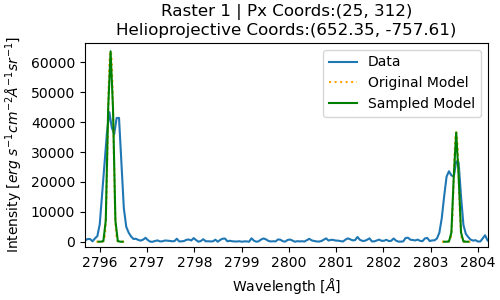
\includegraphics[width=0.49\linewidth]{./02Modelling1D/figs/20180419/inv/bad5.png}
    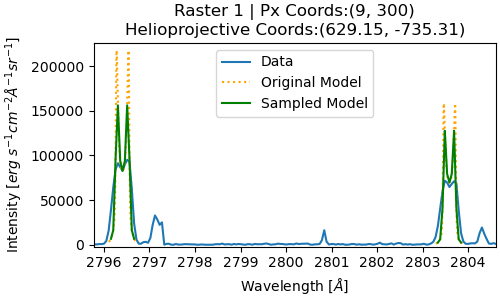
\includegraphics[width=0.49\linewidth]{./02Modelling1D/figs/20180419/inv/bad1.png}
    }
    \resizebox{\hsize}{!}
    {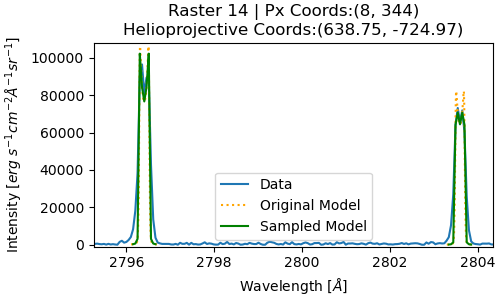
\includegraphics[width=0.49\linewidth]{./02Modelling1D/figs/20180419/inv/good7.png}
    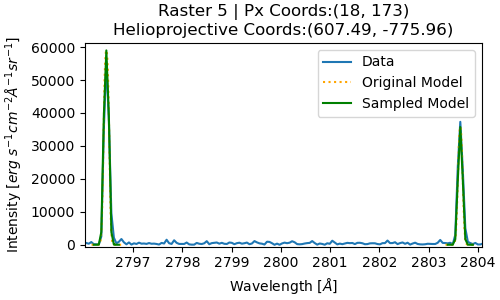
\includegraphics[width=0.49\linewidth]{./02Modelling1D/figs/20180419/inv/good3.png}
    }
    \caption[Four of the twelve matches investigated to set a threshold for the RMS of models found by the algorithm.]{Four of the twelve matches investigated to set a threshold for the RMS of models found by the algorithm. The top two are unsatisfactory matches and the bottom two are satisfactory matches. These plots are from \cite{peat_solar_2021}}
    \label{egpx}
\end{figure}


\begin{figure}
    \centering
    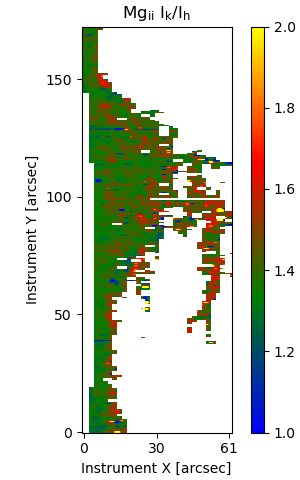
\includegraphics[width=0.3\linewidth]{./02Modelling1D/figs/20180419/kh14.png}
    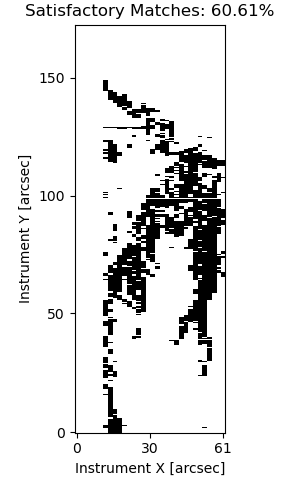
\includegraphics[width=0.3\linewidth]{./02Modelling1D/figs/20180419/goodbad14.png}
    \caption[k/h ratio and satisfactory fits of raster 15. This demonstrates the weak correlation between high k/h ratio and satisfactory fits.]{\textit{Left}: k/h ratio of raster 15. \textit{Right}: Satisfactory fits of raster 15. This demonstrates the weak correlation between high k/h ratio and satisfactory fits. Raster 15 was taken between 18:08 and 18:25 UTC. These plots are from \cite{peat_solar_2021}}
    \label{khandgoods}
\end{figure}

For the results, we will discuss mean pressure and temperature as opposed to the central pressures and temperatures. This gives us a better view of the conditions inside the plasma.
Mean pressure is defined as,
\begin{equation}
    \overline{p}=\frac{1}{M}\int_0^M 4p_c\frac{m}{M}\left(1-\frac{m}{M}\right)+p_{\text{tr}}\hspace{0.1cm}dm,
    \label{meanpresint}
\end{equation}
which evaluates to,
\begin{equation}
    \overline{p}=\frac{2p_{\text{cen}}+p_{\text{tr}}}{3}.
    \label{meanpres}
\end{equation}
Mean temperature is defined as,
\begin{equation}
    \overline{T}=\frac{2}{M}\int_0^{\frac{M}{2}}T_{\text{cen}}+(T_{\text{tr}}-T_{\text{cen}})\left(1-4\frac{m}{M}\left(1-\frac{m}{M}\right)\right)^\gamma dm,
    \label{meantempint}
\end{equation}
which evaluates to
\begin{equation}
    \overline{T}=\frac{2\gamma T_{\text{cen}}+T_{\text{tr}}}{2\gamma+1}.
    \label{meantemp}
\end{equation}
The integral in \eq{meanpresint} is between 0 and $M$ but \eq{meantempint} is between 0 and $M/2$. The prominence is symmetrical around $M/2$, so finding the mean between 0 and $M$ is analogous to the mean between 0 and $M/2$. These bounds are chosen such that they simplify the algebra in the result of the integral.

Figs \ref{mainresults} and \ref{subresults} show the diagnostic results from rRMS. Raster 15 is chosen as the example raster in Fig \ref{subresults} solely due to the field of view being mostly covered by the prominence in this raster.

The mean pressure appears to remain stable over the entire observation, showing small fluctuations between 0.18 and 0.26~dyn~cm$^{-2}$. Towards the centre of the prominence, we find pressures of 1 dyn~cm$^{-2}$. A pressure of 1 dyn~cm$^{-2}$ is at the upper limit of pressures expected to be seen in prominences \citep{labrosse_physics_2010}. However, these high pressures also correlate with areas of unsatisfactory fits. As noted in \chap{Chap:obs}, these are where the most complicated line profiles seem to appear. High pressures can lead to broader line profiles, and this is why rRMS has selected these profiles as a best fit. 1D models are unable to create complicated line profiles like this because the geometry in reality cannot be represented in 1D. The outside and edges of the prominence generally exhibit lower pressures as we move through the PCTR from the core to the low pressure corona \citep{aschwanden_physics_2004}.

As with the mean pressure, the mean temperature also appears stable. On average, the temperature remains between 7800 and 11~500~K. This is consistent with results one would expect. \mgii~h\&k is said to probe the upper photosphere to the upper chromosphere \citep{depontieu_interface_2014} and a prominence is expected to exhibit a range of chromospheric to transition region temperatures. As we approach the edge of the prominence, higher temperatures are observed. This is consistent with where we would expect to observe the PCTR, and therefore higher temperatures, in the plane-of-sky. It could also be that we are intercepting more PCTR material along the line of sight nearer to the edges of the prominence. This would explain why so many fits towards the outside of the prominence have a non-zero gamma value. The arm seen to extend from the prominence near the end of the observations in raster 15 appears to be a hot and tenuous structure reaching temperatures of 4 to 5$\times10^4$~K.

Many of the good fits require a non-zero value of $\gamma$, especially those near the outside of the prominence where higher temperatures are reached. This demonstrates the value of including a PCTR in prominence models. The mean temperatures we find are greater than those found in past \mgii\ studies, such as the study by \citep{zhang_launch_2019}. However, the authors of these past studies did not include a PCTR, they only considered isothermal and isobaric models. In future, we suggest implementing a finer $\gamma$ grid to gain better resolution of the structure of the PCTR surrounding the prominence.

\begin{figure}
    \centering
    \includegraphics*[width=0.25\linewidth]{./02Modelling1D/20180419/outputs/mean_temp/0.png}
    \includegraphics*[width=0.25\linewidth]{./02Modelling1D/20180419/outputs/mean_pres/0.png}
    \includegraphics*[width=0.25\linewidth]{./02Modelling1D/20180419/outputs/gamma/0.png}
    \\
    \includegraphics*[width=0.25\linewidth]{./02Modelling1D/20180419/outputs/mean_temp/11.png}
    \includegraphics*[width=0.25\linewidth]{./02Modelling1D/20180419/outputs/mean_pres/11.png}
    \includegraphics*[width=0.25\linewidth]{./02Modelling1D/20180419/outputs/gamma/11.png}\\
    \includegraphics*[width=0.25\linewidth]{./02Modelling1D/20180419/outputs/mean_temp/14.png}
    \includegraphics*[width=0.25\linewidth]{./02Modelling1D/20180419/outputs/mean_pres/14.png}
    \includegraphics*[width=0.25\linewidth]{./02Modelling1D/20180419/outputs/gamma/14.png}
    \caption[Evolution of mean temperature, pressure, and gamma in the prominence through the main three stages of its evolution, identified in section \ref{20180419main}.]{Evolution of mean temperature, pressure, and gamma in the prominence through the main three stages of its evolution, identified in section \ref{20180419main}. The left and mid columns, and bottom right plot are from \cite{peat_solar_2021}}
    \label{mainresults}
\end{figure}

\begin{figure}
    \centering
    \includegraphics*[width=0.3\linewidth]{./02Modelling1D/20180419/outputs/mnne/14.png}
    \includegraphics*[width=0.3\linewidth]{./02Modelling1D/20180419/outputs/ion_deg/14.png}
    \includegraphics*[width=0.3\linewidth]{./02Modelling1D/20180419/outputs/cmass/14.png} 
    \caption[Mean electron density, ionisation degree, and column mass of the prominence at the culmination of the three stages defined in section \ref{20180419main}.]{Mean electron density, ionisation degree, and column mass of the prominence at the culmination of the three stages defined in section \ref{20180419main}. These plots are from \cite{peat_solar_2021}}
    \label{subresults}
\end{figure}


The column mass found suggests that the extensions of the prominence are of relatively low mass. Where we find unsatisfactory matches, the mass density is seen to be much higher. We also see \ha\ emission in this area, and \ha\ is known to require denser areas to be seen. The unsatisfactory fits here are mainly due to the single slab nature of the 1D modelling. As discussed, we see several threads along the line of sight in this area. A single slab model can only apply, when there are several threads, if the threads are co-moving, resulting in a single line profile. The arm seen to extend near the end of the observations is seen to be of relatively low mass. This explains the single peaked profiles seen in the arm. The intensity of the line core of \mgii~h\&k is anticorrelated with optical depth, which further explains the correlation between single peaked profiles and low mass density \citep{leenaarts_formation_2013}.

On the whole, the prominence appears to have an electron density less than $0.6\times10^{11}$~cm$^{-3}$, with few areas exceeding $1\times10^{11}$~cm$^{-3}$ (Fig. \ref{subresults}). The arm is seen to be of comparatively low electron density, although it is high temperature. However, it is also of low pressure, which can explain this disparity. 

Ionisation degree is defined by the mean number density of \ion{H}{ii} ($n_\text{HII}$) to the mean number density of \ion{H}{i} ($n_\text{HI}$) \citep{tandberg-hanssen_nature_1995}. Past works have assumed that the mean number of electrons ($n_\text{e}$) is equal to the mean number of protons ($n_\text{p}$), which is equal to the mean number density of \ion{H}{ii}. The mean number of \ion{H}{i} is also thought to be dominated by the mean number density of ground state Hydrogen ($n_\text{H0}$), such that,

\begin{equation}
    \frac{n_\text{HII}}{n_\text{HI}}\approx\frac{n_\text{p}}{n_\text{H0}}\approx\frac{n_\text{e}}{n_\text{H0}}.
\end{equation}

However, the assumption that $n_\text{e}\approx n_\text{p}=n_\text{HII}$ does not hold in PROM as not all of the electrons are liberated from \ion{H}{i}. There is a fixed percentage contribution from other species, mainly helium. These `non-hydrogen' electrons contribute greatly to $n_\text{e}$ at high temperatures. The right panels of Fig. \ref{iondeg} shows how this assumption breaks down at higher temperatures. Above 30~000~K, $n_\text{HII}$ is overestimated by 20\% by this metric. So here, we focus on the definition from \cite{tandberg-hanssen_nature_1995}. Parts of the prominence show a very high ionisation degree when compared to past studies. \cite{vial_solar_1998} stated that the ionisation degree in a prominence does not dramatically change with temperature, given that the density is low. This statement was grounded in studies by \cite{gouttebroze_hydrogen_1993} and \cite{heinzel_theoretical_1994}. However, these studies did not consider temperatures above 15~000~K and did not include a PCTR. The left of Fig. \ref{iondeg} shows that above this temperature, ionisation degree increases exponentially. Additionally, at this temperature, the overestimation of $n_\text{HII}$ when it is assumed to be equal to $n_\text{e}$, is only approximately 7\%. This could very easily go unnoticed. In past studies using isothermal and isobaric models, ionisation degree was not thought to rise above 10. However, areas of high ionisation degree (see Fig. \ref{subresults}), strongly correlate with areas of non-zero $\gamma$. This demonstrates that the inclusion of a PCTR can dramatically influence the value of the ionisation degree.



\begin{figure}
    \centering
    \includegraphics*[width=0.4\linewidth]{./02Modelling1D/figs/20180419/ideg_temp_new.png}
    \includegraphics*[width=0.4\linewidth]{./02Modelling1D/figs/20180419/excess_electrons.png}
    \caption[Exponential rise in ionisation degree above 30~000~K and how the assumption that $n_\text{e}\approx n_\text{HII}$ breaks down at high temperatures.]{\textit{Left}: Exponential rise in ionisation degree above 30~000~K. \textit{Right}: How the assumption that $n_\text{e}\approx n_\text{HII}$ breaks down at high temperatures. These plots are from \cite{peat_solar_2021}.}
    \label{iondeg}
\end{figure}

As an added consequence of rRMS, we also obtain line of sight Doppler velocities as we recover the pixel location in wavelength where the lowest RMS is found. This allows us to create Doppler maps which can be compared to the Doppler maps recovered from the quantile method shown in \sect{velsect} to demonstrate that the algorithm is functioning correctly. The resolution of these line core shifts is approximately 2.7~km~s$^{-1}$. This number is from the minimum measurable line core shift by the procedure. This is equal to the wavelength resolution of the observations divided by the number of sub-pixels plus one. 

Fig. \ref{vels} shows the line core shift found via the quantile method and that recovered by rRMS. The Doppler maps of the top of this figure appear to qualitatively agree. With the other diagnostics, there is uncertainty in the recovered value where unsatisfactory fits are found. While these models do not represent the conditions of the prominence plasma, the fit found by the procedure should still find a good measure of the line core shift; regardless of how bad the fit is. This is because the lowest RMS is mostly found when the model profile is centred on the data profile. Due to this, we can reasonably trust the line core shifts recovered by rRMS, even where unsatisfactory fits are found.
The histograms for the recovered line core shift from rRMS in Fig. \ref{vels} have fewer bins than that of the line core shift measured by the quantile method. This is because the velocity resolution of the results of the quantile method is essentially infinite, but the resolution of the recovered line core shifts is only 2.7~km~s$^{-1}$, as previously discussed. Both of these distributions approximate well to Gaussians. The fit to the histograms obtained via the quantile method are centred on a line core shift of 8.20~km~s$\pm$5.98\kms and 5.20$\pm$6.61\kms for \mghk, respectively. Those recovered via rRMS are centred on a line core shift of 5.3~km~s$^{-1}$ and 5.6~km~s$^{-1}$ with standard deviations of 9.8~km~s$^{-1}$ and 10.2~km~s$^{-1}$ for \mghk, respectively. Due to the limited resolution of the line core shift recovered by rRMS, a value of $\pm1.35$~km~s$^{-1}$ is given as an estimate of the uncertainty of these values. This value is half of the minimum recoverable line core shift by rRMS. The central line core shift of \mgii~k measured by the quantile method is within the uncertainty of the line core shift recovered from rRMS. However, this is not true with the line core shift of \mgii~h. This is believed to be due to the asymmetry bias discussed in \sect{velsect} but it is not clear why only \mgii~h is affected by this. This could be a result of \mgii~h generally having a smaller line width compared to \mgii~k or opacity effects.

\begin{figure}
    \centering
    \includegraphics*[width=0.4\linewidth]{./02Modelling1D/figs/20180419/quantdopp.png}
    \includegraphics*[width=0.4\linewidth]{./02Modelling1D/figs/20180419/rolldopp.png}\\
    \includegraphics*[width=0.3\linewidth]{./02Modelling1D/figs/20180419/hvelocities.png}
    \hspace{1cm}
    \includegraphics*[width=0.3\linewidth]{./02Modelling1D/figs/20180419/hvelocitiesfound.png}\\
    \includegraphics*[width=0.3\linewidth]{./02Modelling1D/figs/20180419/kvelocities.png}
    \hspace{1cm}
    \includegraphics*[width=0.3\linewidth]{./02Modelling1D/figs/20180419/kvelocitiesfound.png}
    \caption[Doppler velocities found using the quantile method and Doppler velocities recovered from rRMS.]{\textit{Left:} Doppler velocities found using the quantile method. \textit{Right:} Doppler velocities recovered from rRMS. The dashed line represents a line core shift of 0~km~s$^{-1}$ and the orange line is a Gaussian fit. These plots are from \cite{peat_solar_2021}}
    \label{vels}
\end{figure}
\newpage
\section{Cross Root Mean Squared (xRMS)}
\label{xrms}
\textit{The content of this section is based on work presented in Peat et al. (in prep.).}

Since the publication of \cite{peat_solar_2021}, rRMS has been modified and renamed. It is now called Cross(-correlation) Root Mean Square Difference (xRMS). The main difference between rRMS and xRMS is that the `roll' is predetermined by a cross-correlation, hence the name change. A cross-correlation is naturally produced when attempting to minimise (or maximise) a mean square \citep{elliott_handbook_1987}, and therefore also when minimising a root mean square. Additionally, \cite{brown_doppler_2016} demonstrated that a cross correlation could be employed to find the line core shift of the Lyman lines in solar flares. As the rolling aspect of rRMS was essentially measuring the line core shift, it was decided that computation time could be greatly improved by the introduction of a cross-correlation to predetermine the line core shift. After the cross-correlation is computed, the line profiles are then rolled to their respective line core shift, and the RMS was measured. This improved the run time by a factor of approximately 10. This final roll was then determined to be the new bottleneck to the algorithm, and so this was also improved upon. As a model profile is being matched, a reference padded profile (rpp) is created. This rpp is the considered model profile padded on both sides by zeroes the length of the difference between the length of the data array and the model array. This allows us to take slices of the rpp identical to the result of a would-be roll. Taking slices of an array does not create a new array, and only a new pointer (or reference in Python) which is considerably faster. This removed the need for rolled model arrays to be created, improving the run time by a further factor of approximately 2. xRMS and rRMS give the same results, but due to the optimisations introduced, xRMS is much faster. Running the same 1007 model grid on the same data as presented in \cite{peat_solar_2021}, but using xRMS, on the same dual socket motherboard machine with two Intel Xeon E5-2697 v4s, gives a wall time of approximately 6 minutes and 30 seconds, and a CPU time of 1 hour and 57 minutes. Due to this great improvement in computation time, this allows us to use a much larger grid of models.

In addition to the faster computation time, xRMS supplies us with an estimate of the errors on our inversion. It does this by saving the 20 next best fitting models alongside the best fitting model. Then, of these secondary models, it removes those whose RMS is lower than the threshold value as defined previously. This is followed by finding the maximum difference between the `best fit' diagnostics and the remaining good secondary fit diagnostics. These values are then divided by the `best fit' value to recover fractional errors. This is done to give a better indication of the range of values of good, but not best, fits that can be found. These fractional errors are how the uncertainty will be presented in plots later in this section. This maximum difference which makes up the error need not be from the same model. To be conservative, the error is the greatest difference produced by any of the secondary models. For example, a pixel may not necessarily use the same model for its pressure uncertainty and temperature uncertainty.
 
\subsection{Prominence of 2018 04 19: Revisited}

To exhibit the efficacy of the new algorithm, we will use the prominence used to demonstrate rRMS in \sect{20180419} to illustrate how our matches improve with a greater set of models.

As mentioned above, here can we employ a much larger grid of models than used previously due to the increase in computation offered by xRMS. Additionally, we introduce the parameter $v_\text{rad}$. This is the radial (outward) velocity. This allows us to introduces Doppler dimming into our models. In total, there are 23~940 models in our new grid, this includes the previous 1007 models used in \sect{20180419}. See Table \ref{23940table} for the range of parameters present in the models. Please note that these values are not all uniquely combined.
\begin{table}[]
    \centering
    \begin{tabular}{ccc}
    \hline\hline
    Parameter  & Unit                & Value                                                                                                                                                        \\ \hline
    $T_\mathrm{cen}$  & K                   & \begin{tabular}[c]{@{}c@{}}6000, 8000, 10~000, 12~000, 15~000,\\ 20~000, 25~000, 30~000, 35~000, 40~000\end{tabular} \\
    $T_\mathrm{tr}$   & K                   & 100~000                                                                                                                                                 \\
    $p_\mathrm{cen}$  & dyne~cm$^{-2}$ & 0.01, 0.02, 0.05, 0.1, 0.2, 0.5, 1                                                                                                                           \\
    $p_\mathrm{tr}$   & dyne~cm$^{-2}$ & 0.01                                                                                                                                                         \\
    Slab width & km                  & 45-124~100                                                                                                                                              \\
    M          & g~cm$^{-2}$    & $3.7\times10^{-8}-5.1\times10^{-4}$                                                                                                                          \\
    $v_{T}$    & km~s$^{-1}$    & 5, 8, 13                                                                                                                                                     \\
    $v_\mathrm{rad}$  & km~s$^{-1}$    & \begin{tabular}[c]{@{}c@{}}0, 2, 4, 6, 8, 10, 20, 40,\\ 60, 80, 100, 150, 200\end{tabular}                                                                   \\
    H          & km                  & 10~000, 30~000, 50~000                                                                                                                        \\
    $\gamma$   &                     & 0, 2, 4, 5, 10                                                                                                                                               \\ \hline
    \end{tabular}
    \caption[The considered model parameters to be used in xRMS.]{The considered model parameters to be used in xRMS. Not all of these parameters are uniquely combined; there are 23940 total model profiles. Amongst these models are the original 1007 from \sect{20180419}.}
    \label{23940table}
\end{table}
The results from xRMS can be seen in \fig{20180419rresults}. As the grid of models was increased, even though the previous 1007 models were coarsely separated, the cut off value did not change. After investigating the same 12 profiles, the cut off value was once again decided to be 15000. We now achieve 55.14\% (39450/71548) satisfactory matches. The total number of pixels is different with xRMS than rRMS as the updated version of the filter discussed in \sect{20180419main} is used in xRMS but not in rRMS. 

As noted in \sect{20180419main}, the prominence displays an array of interesting line profiles. With these new diagnostics, we can explore some of them in more detail. In \fig{2structs}, shows one of the unsatisfactory matches. However, it could be argued that this is satisfactory as this is not a double peaked profile, but two structures. The main drawback of this method is that it assumes single structures along the line of sight. In the future, it could be possible to allow for multi-structure solutions, but this would almost double the required computation time, so this method may be reaching its limit. From the matching model, we can see that the optical depth of the fit structure is $0.97$ and $1.90$ for \mgiihk{}, respectively, and the k/h ratio is approximately $1.71$. Therefore, it is safe to say that this structure is mostly optically thin. In this case, we would be justified in trying to fit a second peak as if the first was not there. From just looking at the line profiles and the model line profiles, I would expect a similar, if not the same, model to fit this secondary peak. There are many other line profiles like this in the prominence, but this is the most apparent example. In \sect{2dinvert} we attempt to invert this spectrum using stacked 2D models.

\begin{figure}
    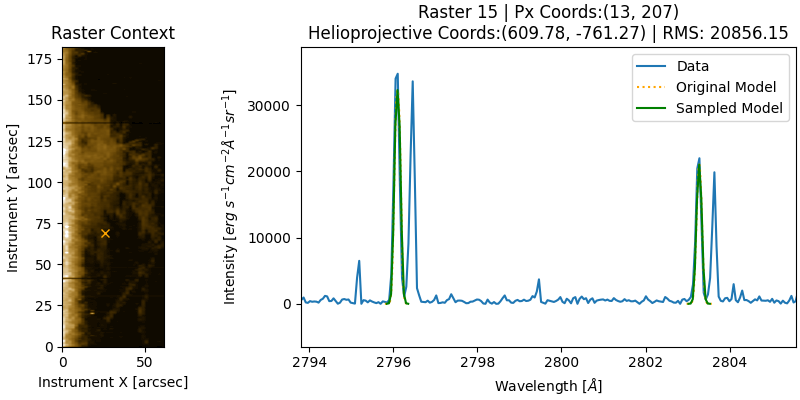
\includegraphics[width=\linewidth]{./02Modelling1D/figs/lineprofs/r15y13x207.png}
    \caption[The \mgiihk{} spectra from the raster taken from 18:25:09~UTC.]{The \mgiihk{} spectra from the raster taken from 18:25:09~UTC. The orange cross indicates the location this spectra is taken from. The model found to match by xRMS here has the following parameters, $T=8000$~K, $p=0.02$\dyncm{}, Slab Width$=200$~km, $v_T=8$\kms{}, $H=10000$~km, $v_\text{rad}=80$\kms{}, and $\gamma=0$, with associated Doppler velocities of $v_{dh}=-27.0$\kms{} and $v_{dk}=-27.0$\kms{}.}
    \label{2structs}
\end{figure}

\fig{similar} shows two spectra of similar parameters. The difference in microturbulent velocity is apparent due to their difference in line width. These two spectra come from different parts of the prominence. The top panel is from the middle of the main extension, and the bottom panel from one of the smaller extensions from the main body. Although they are in very different locations, they both have the same central temperature, and mean temperature (32000K). Their pressures, however, are different. The pressure of the main extension is four times higher than that of the smaller extension. This is not surprising, as the main extension is comprised of a larger volume than that of the smaller extension. Their measure of radial velocity can also tell us more about the velocity perpendicular to the solar limb. The main moving faster than the small extension. This is consistent with observation, as the smaller extensions are seen to move slower than the main extension in SJI movies.
\begin{figure}
    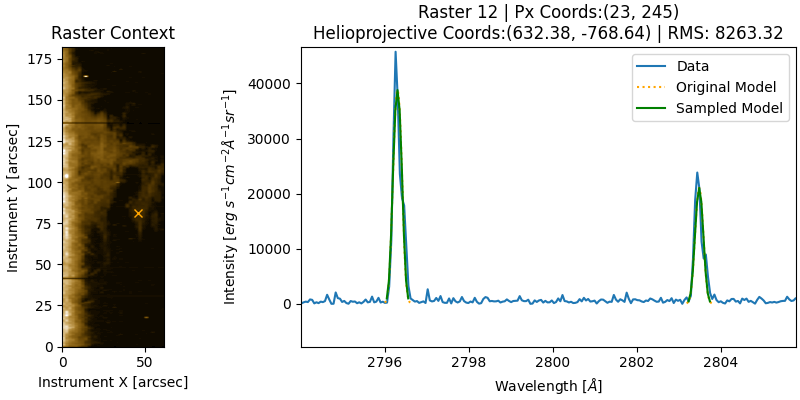
\includegraphics[width=\linewidth]{./02Modelling1D/figs/lineprofs/r12y23x245.png}
    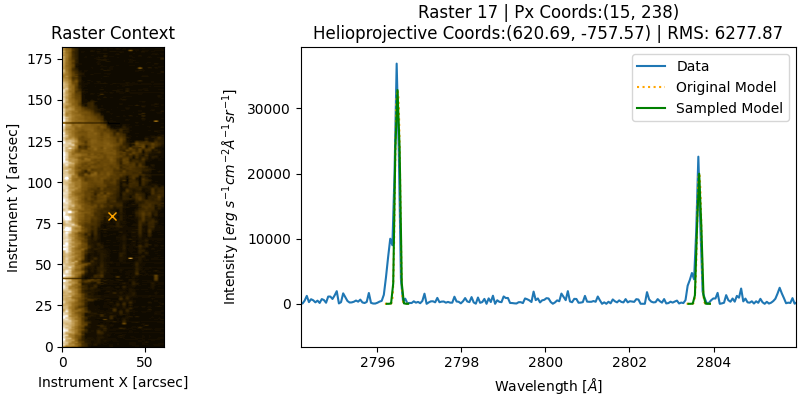
\includegraphics[width=\linewidth]{./02Modelling1D/figs/lineprofs/r17y15x238.png}
    \caption[The \mgiihk{} spectra from two raster taken at different times, 17:34:54~UTC and 18:58:40~UTC]{The \mgiihk{} spectra from two raster taken at different times, 17:34:54~UTC and 18:58:40~UTC for the top and bottom panel respectively. The orange cross indicates the location this spectra is taken from. The model found to match by xRMS here has the following parameters, I will omit the PCTR variables as they can only be one number (see Table \ref{23940table}), \\\textit{Top}: $T_\text{cen}=15000$~K, $p_\text{cen}=0.20$\dyncm{}, Slab Width$=1148$~km, $v_T=13$\kms{}, $H=10000$~km, $v_{\text{rad}}=80$\kms{}, and $\gamma=2$. With associated Doppler velocities of $v_{dh}=5.22$\kms{} and $v_{dk}=5.23$\kms{}. \\\textit{Bottom}: $T_\text{cen}=15000$~K, $p_\text{cen}=0.05$\dyncm{}, Slab Width$=2640$~km, $v_T=5$\kms{}, $H=50000$~km, $v_{\text{rad}}=60$\kms{}, and $\gamma=2$. With associated Doppler velocities of $v_{dh}=13.84$\kms{} and $v_{dk}=13.88$\kms{}.}
    \label{similar}
\end{figure}

As a whole, in comparison to our results with a smaller set of models, we see a much more striking temperature structure. Compared to the mean temperatures seen in the previous result, they are much higher here. The temperature structure seems more homogeneous, but the highest temperatures are still found in the arm.
The fractional errors, however, are mostly between 0 and 3. The distribution of recovered pressures is also different. The higher microturbulent velocities have allowed a better match at the centre of the prominence than those of high pressure. However, we still do not find satisfactory matches in this area due to the multiple structures seen in many pixel locations. The areas we find good matches in correlate with areas of lower pressure. Before, we had many regions in the prominence where $\gamma=10$, but now there are none, with $\gamma=4$ and $\gamma=2$ appearing in these high temperature areas. However, the uncertainty shows that gamma could be up to two times higher in the majority of the regions where it was previously found to be 10. The blank spaces in the gamma uncertainty map are where an isothermal and isobaric model was found to be the best fit. Calculating the fractional difference in these locations is meaningless, and so they are discarded. Like before, our satisfactory matches correlate weakly with high k/h ratio. Our lowest errors (bottom of \fig{20180419rresults}) correlate with both of these graphs. 

\begin{figure} 
    \centering
    \includegraphics*[width=\linewidth]{./02Modelling1D/20180419r/fullfig.png}
    \caption[Mean Temperature, Pressure, and Gamma Results from xRMS for the prominence of 2018 04 19]{Mean Temperature, Pressure, and Gamma results for the middle of the three stages identified in the prominence. \textit{Left}: Mean temperature. \textit{Mid}: Mean pressure. \textit{Right}: Gamma. \textit{Top}: The main result. \textit{Bottom}: Their fractional uncertainties.}
    \label{20180419rresults}
\end{figure}

However, presenting these as a traditional plus/minus uncertainty is perhaps not best, as 1D inversions like this can be shown to have degenerate solutions. In test 1D Markov Chain Monte Carlo (MCMC) inversions of a set of simulated (and known-parameter) \mgiihk{} line profiles show that posterior likelihoods tend to display multimodal distributions \citep{osborne_notitle_2022}\footnote{This was explored using profiles from Promweaver: \href{https://github.com/Goobley/Promweaver}{https://github.com/Goobley/Promweaver}}. The introduction of more spectral lines from different species may solve this issue of degeneracy, but has not yet been explored. 

Even though we increased our model set by a factor of 24, we only increased our matches by approximately 6\%. Although this increase is small, some parts of the prominence now have better matches than before. This increase in satisfactory matches is owed to the increase in the number of models in the grid. However, the main problem with a grid search method is that your algorithm can only perform as well as your grid represents the plasma conditions, the grid can be continually increased, but that does not mean that your matches will improve. There is only so much 1D models can do on their own. Even though we cannot satisfactorily probe the centre of the prominence with these models, we are able to diagnose the area surrounding the prominence. This gives us insight into the enigmatic PCTR. It is the reason that we find larger than expected ionisation degrees, and high temperature. The continued study of transition region lines, such as \mgiihk{}, can lead to a better understanding of how the PCTR is structured.  



\section{Concluding Remarks}

1D modelling can be a very useful tool to understand how the internal plasma parameters of a solar prominence affect the shape of its observed line profiles.
However, they are limited in their use to diagnose the internal plasma parameters from observation. Their 1D nature means that they cannot easily model the mulithreaded nature of many prominences. Additionally, they can be shown to have degeneracies in their solutions when fitting to one species. The introduction of multiple species may solve this issue, but this topic remains unexplored. Despite these limitations, they can (and have) shown us that the PCTR is very important when it comes to \mgiihk{} modelling. This is likely due to their high optical thickness which only allows us to probe the surface of the prominence and not penetrate too deeply into the body. The seemingly degenerate nature of this problem of inverting prominence atmospheres using 1D modelling motivates us to explore the applications and interpretation to be gleaned from 2D modelling. However, in future, coordinated observations of different line profiles, such as \mgiihk{} and \ha{}, could be used to further constrain the atmosphere and may solve this degeneracy problem.